\section{Formal Results}
\label{sec:formal-results}

%\begin{itemize}
%	\item Results that we rely on (petri nets, semilinear sets)
%	\item The base algorithm described in math (without any optimizations)
%	\item Time complexity
%	\item proof for correctness of bidirectional pruning
%	\item mathematical description of optimizations
%\end{itemize}




\subsection{The Algorithm (without Optimizations)}

Given a network system, defined as \(\mathcal S= (G, L, \mathit{REQ},  \mathit{RESP}, g_0, \delta, \mathit{req}, \mathit{resp})\), our decision procedure runs the following steps:  

%\begin{enumerate}
%	\item  
\medskip
	\noindent
	\textbf{Step 1: Serializability automaton.} 
	We define the following NFA 
	\(
	\mathcal A_{\mathrm{ser}}(\mathcal S)=(Q,\Sigma,\delta^A,q_0,F)
	\), with
	\( Q=G,\;F=G,\;q_0=g_0,
	\)
	over the alphabet of all request/response pairs
	\(
	\Sigma=\{({\color{ForestGreen}\blacklozenge_{\mathit{req}}}/{\color{red}\blacklozenge_{\mathit{resp}}})
	\mid {\color{ForestGreen}\blacklozenge_{\mathit{req}}}\in\mathit{REQ},\;
	{\color{red}\blacklozenge_{\mathit{resp}}}\in\mathit{RESP}\}.
	\)
%	
%	\todo{old}
%	We define an NFA
%	\[
%	\mathcal A_{\mathrm{ser}}(\mathcal S)
%	= \bigl(Q,\Sigma,\delta,q_0,F\bigr),
%	\quad
%	Q = G,\quad F = G \;\;(\text{global states}),\quad
%	q_0 = g_0 \;\;(\text{initial state}),
%	\]
%	\[
%	\Sigma
%	= \Bigl\{
%	({\color{ForestGreen}\blacklozenge_{\mathit{req}}}\,/\,%
%	{\color{red}\blacklozenge_{\mathit{resp}}})
%	\;\Big|\;
%	{\color{ForestGreen}\blacklozenge_{\mathit{req}}}\in\mathit{REQ},\;
%	{\color{red}\blacklozenge_{\mathit{resp}}}\in\mathit{RESP}
%	\Bigr\}.
%	\]
%
Each transition of the NFA corresponds to a single character, i.e., a single request/response pair:
\(
\delta^A \subseteq Q \times \Sigma \times Q,
\quad q \xrightarrow{{\color{ForestGreen}\blacklozenge_{\mathit{req}}}/{\color{red}\blacklozenge_{\mathit{resp}}}} q'
\),
%old
%\(
%\delta \;\subseteq\; Q \times \Sigma_{	{\color{ForestGreen}\blacklozenge_{\mathit{req}}}\,/\,%
%	{\color{red}\blacklozenge_{\mathit{resp}}}} \times Q,
%\quad
%\bigl(q \xrightarrow{%
%	{\color{ForestGreen}\blacklozenge_{\mathit{req}}}\,/\,%
%	{\color{red}\blacklozenge_{\mathit{resp}}}%
%} q'\bigr),
%\)
%
%\;\Longleftrightarrow\;
%\begin{array}{l}
iff network system $\mathcal S$ is in global state $q$ and issues a request
$	{\color{ForestGreen}\blacklozenge_{\mathit{req}}}$, then upon some \textit{full serial execution} of $	{\color{ForestGreen}\blacklozenge_{\mathit{req}}}$ the network system finally transitions to the global state  $q'$ and returns to the user the response $	{\color{red}\blacklozenge_{\mathit{resp}}}$.
%\end{array}
%\]
%
%
%
%
%
%
%\begin{array}{l}
%	\mathcal S \text{ at global state } q
%	\;\text{issues}\;
%	{\color{ForestGreen}\blacklozenge_{\mathit{req}}},\\[0.5ex]
%	\text{after full completion of the request, it receives}\;
%	{\color{red}\blacklozenge_{\mathit{resp}}},\\[0.5ex]
%	\text{arriving at global state } q'
%\end{array}
%\]
%
%	
The NFA's language
	\(L(\mathcal A_{\mathrm{ser}}(\mathcal S))\subseteq\Sigma^*\) is the set of
	request/response traces induced by serial executions, from any reachable global state.
	Hence, by definition, applying the Parikh image on this regular language induces the (infinite) set of all (order-less) multisets of request/response pairs that are obtained by serial executions:
	\(
	\mathsf{Ser}(\mathcal S)
	\;=\;
	\mathsf{Parikh}\bigl(L(\mathcal A_{\mathrm{ser}}(\mathcal S))\bigr)
	\;\subseteq\;\mathbb N^{\Sigma}.
	\)
%	Finally,
%	\(
%	q_0 = g_0
%	\quad\text{(the initial global state of the NS)}
%	\).
	
	
%	\smallskip
\begin{tcolorbox}[colback=black!5!white, colframe=black, boxrule=1pt]
	\textbf{Example.} For Listing~\ref{lst:MotivatingExample2NonSer}, the network system in Fig.~\ref{fig:code2ExampleNS} gives rise to the Serial NFA that is presented in Fig.~\ref{fig:code2ExampleNFA}.
	%
	A trace of request/response pairs is accepted by the NFA iff there exists a serial execution of the network system that induces it.
	%	
In this case, serial executionsinduce only ({\color{ForestGreen}$\blacklozenge_\text{main}$}/{\color{red}$\blacklozenge_1$}), and the only reachable global state is [\texttt{X=0}].
%	Due to the aforementioned construction, a string of request/response pairs is accepted by the NFA iff there exists a serial execution of the NS that induces it.
%
%	As the states encode the global variable values, and the edges encode request/response pairs for all serial executions, the  
%Specifically, in this case --- serial executions can only produce request/response pairs of the type ({\color{ForestGreen}$\blacklozenge_\text{main}$/{\color{red}$\blacklozenge_1$}}). Furthermore, the only global state reachable in serial executions, is [\texttt{X=0}]. 
	%
%	Intuitively, this corresponds to [\texttt{X=0}] being the initial global state, as well as the system's global state after every single packet exits the network in a serial execution.
	\end{tcolorbox}
	%
%	\begin{figure}[!htbp]
%		\centering
%		% 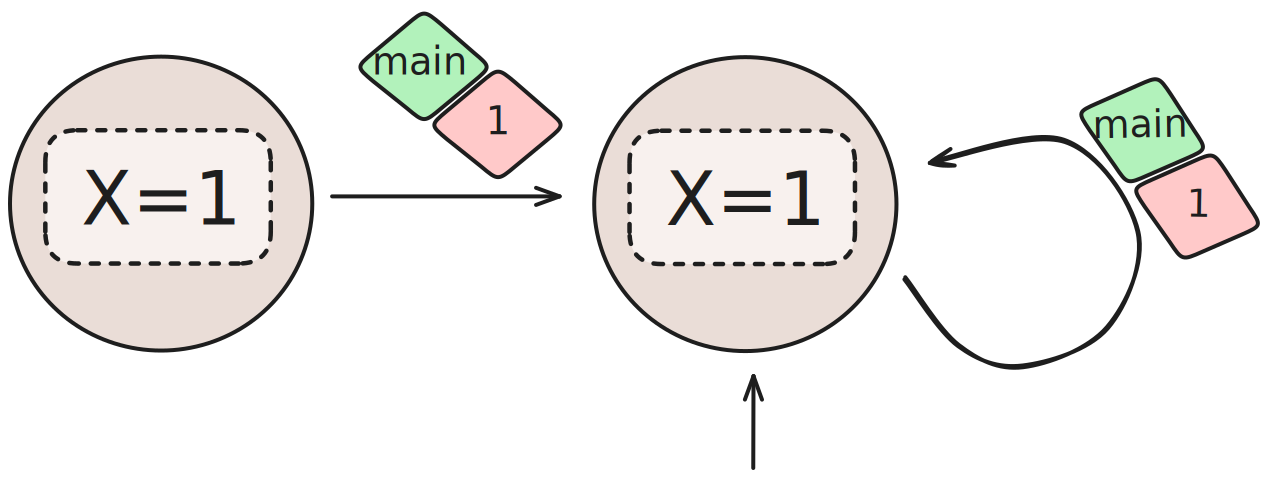
\includegraphics[width=0.48\textwidth,trim=0 0 0 0,clip]{plots/code_2_NFA_v3.pdf}
%		
%		\begin{tikzpicture}[
%			->,>=stealth,
%			thick,
%			node distance=2.5cm,
%			state/.style={
%				draw=black,
%				line width=0.8pt,
%				fill=blue!10,
%				rectangle,
%				rounded corners=1pt,
%				inner sep=2pt,
%				font=\small
%			},
%			every node/.style={font=\small}
%			]
%			% States using the same notation as section 3
%			\node[state] (X1) {\texttt{X=1}};
%			\node[state, right of=X1] (X0) {\texttt{X=0}};
%			
%			% Initial state arrow
%			\draw[->] ([yshift=-0.4cm]X0.south) -- (X0.south);
%			
%			% Transitions with proper colored notation from the paper
%			\draw[->] (X1) -- node[above] {${\color{ForestGreen}\blacklozenge_{\mathrm{main}}}/{\color{red}\blacklozenge_1}$} (X0);
%			\draw[->] (X0) edge[loop right] node[right] {${\color{ForestGreen}\blacklozenge_{\mathrm{main}}}/{\color{red}\blacklozenge_1}$} (X0);
%		\end{tikzpicture}
%		
%		\caption{Serial NFA of Listing~\ref{lst:MotivatingExample2NonSer}.}
%		\label{fig:code2ExampleNFA}
%	\end{figure}
	
	\begin{figure}[!htbp]
		\centering
		
		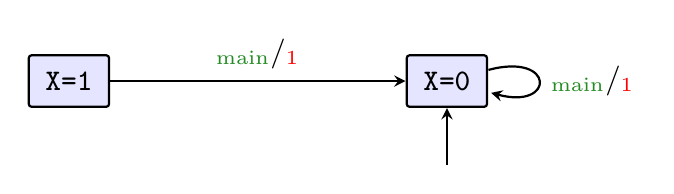
\begin{tikzpicture}[
			scale=1.2, transform shape,  % Scales the entire diagram and text
			->,>=stealth,
			thick,
			node distance=4cm, % Increased distance for better spacing
			state/.style={
				draw=black,
				line width=0.8pt,
				fill=blue!10,
				rectangle,
				rounded corners=1pt,
				inner sep=5pt, % Slightly more padding
				font=\small
			},
			every node/.style={font=\small}
			]
			% States using the same notation as section 3
			\node[state] (X1) {\texttt{X=1}};
			\node[state, right of=X1] (X0) {\texttt{X=0}};
			
			% Initial state arrow
			\draw[->] ([yshift=-0.6cm]X0.south) -- (X0.south);
			
			% Transitions with proper colored notation from the paper
			\draw[->] (X1) -- node[above] {${\color{ForestGreen}\blacklozenge_{\mathrm{main}}}/{\color{red}\blacklozenge_1}$} (X0);
			\draw[->] (X0) edge[loop right] node[right] {${\color{ForestGreen}\blacklozenge_{\mathrm{main}}}/{\color{red}\blacklozenge_1}$} (X0);
		\end{tikzpicture}
		
		\caption{Serial NFA of Listing~\ref{lst:MotivatingExample2NonSer}.}
		\label{fig:code2ExampleNFA}
	\end{figure}

	
%	\begin{wrapfigure}{r}{0.50\textwidth}  % “r” = right, width = 0.5\textwidth
%		\centering
%		% 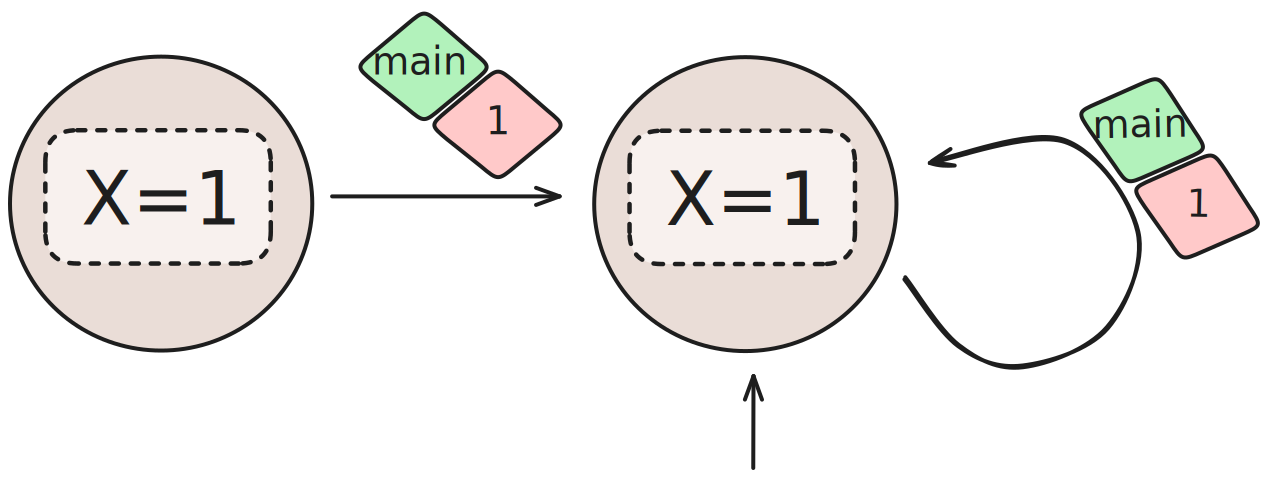
\includegraphics[width=0.48\textwidth,trim=0 0 0 0,clip]{plots/code_2_NFA_v3.pdf}
%		
%		\begin{tikzpicture}[
%			->,>=stealth,
%			thick,
%			node distance=2.5cm,
%			state/.style={
%				draw=black,
%				line width=0.8pt,
%				fill=blue!10,
%				rectangle,
%				rounded corners=1pt,
%				inner sep=2pt,
%				font=\small
%			},
%			every node/.style={font=\small}
%			]
%			% States using the same notation as section 3
%			\node[state] (X1) {\texttt{X=1}};
%			\node[state, right of=X1] (X0) {\texttt{X=0}};
%			
%			% Initial state arrow
%			\draw[->] ([yshift=-0.4cm]X0.south) -- (X0.south);
%			
%			% Transitions with proper colored notation from the paper
%			\draw[->] (X1) -- node[above] {${\color{ForestGreen}\blacklozenge_{\mathrm{main}}}/{\color{red}\blacklozenge_1}$} (X0);
%			\draw[->] (X0) edge[loop right] node[right] {${\color{ForestGreen}\blacklozenge_{\mathrm{main}}}/{\color{red}\blacklozenge_1}$} (X0);
%		\end{tikzpicture}
%		
%		\caption{Serial NFA of Listing~\ref{lst:MotivatingExample2NonSer}.}
%		\label{fig:code2ExampleNFA}
%	\end{wrapfigure}
	%
	%
	%Intuitively, this corresponds to the Listing~\ref{lst:MotivatingExample2NonSer} program updating [X:=1] as an intermediate assignment before yielding.
	
	
	
%\medskip
\noindent
%	\item 
	\textbf{Step 2: Interleaving Petri net.}
%	
Next, we translate the network system into a Petri net \(N_{\mathrm{int}}(\mathcal S)\). Each \textit{non-sink place} of the Petri net represents either a global state assignment or a local states of in-flight packets. Each \textit{sink place} represents request/response pairs of terminated packets.
%
The \textit{transitions} between states are defined to correspond to the \(\delta\), \(req\), and \(resp\) mappings of the network system. We note that the \(req\) transitions can fire without any input tokens in order to correspond to external spawning of arbitrarily-many requests.
%
Finally, we define \(M_0\) to be an initial marking encoding a single token in the non-sink place corresponding to \(g_0\), i.e., the initial global state of the network system.
%
This construction is formalized in full in  Appendix~\ref{appendix:NS-to-PN-formulation}, and guarantees that each multiset of all markings \(M\) (with \(M_0 \xrightarrow{}^{*} M\)) when projected (via \(\pi\)) to the sink places, corresponds to a multiset of (${{\color{ForestGreen}\blacklozenge_{\mathit{req}}}/{\color{red}\blacklozenge_{\mathit{resp}}}}$) pairs, as induced by a network system interleaving, i.e., \(\mathsf{Int}(\mathcal S)=\{\pi(M) \mid M \in R(N_{\mathrm{int}}(\mathcal S))\}\).



\begin{tcolorbox}[colback=black!5!white, colframe=black, boxrule=1pt]
	\textbf{Example.}
%	\textit{Notation.}
Continuing our running example, the network system induces the Petri net presented in Fig.~\ref{fig:code2ExamplePN}, encoding all possible interleavings. The places \textcolor{blue}{$P_2$} and \textcolor{blue}{$P_3$} respectively correspond to the global states \textcolor{blue}{[X=1]} and \textcolor{blue}{[X=0]}, and places $P_1$, $P_4$, $P_5$, and $P_6$ correspond to the local states of in-flight requests, i.e., the assignments to each request’s local variables, coupled with the remaining \toolname{} program code to execute. Similarly, places \textcolor{red}{$P_7$} and \textcolor{red}{$P_8$} correspond to responses {\color{red}$\blacklozenge_1$} and {\color{red}$\blacklozenge_0$}, respectively. Thus, each token models either an active (in-flight) request, a completed request/response pair, or --- when the token resides in a place denoting the global state --- the current global state of the network system. Finally, transitions are induced by the network system’s mappings ($\delta/req/resp$): they either advance the program by a single step (e.g., \(t_2,t_3,t_4,\) and \(t_5\), based on $\delta$), represent external spawning of a new request (e.g., transition $\textcolor{ForestGreen}{t_1}$, which corresponds to request {\color{ForestGreen}$\blacklozenge_{\mathrm{main}}$} based on $req$),
or return a response (e.g., transitions $\textcolor{red}{t_6}$ and $\textcolor{red}{t_7}$, based on $resp$).
\end{tcolorbox}

%Finally, the NS gives rise to the PN in Fig.~\ref{fig:code2ExamplePN}, encoding all possible interleavings.
%%
%The places represent either the global state
%(e.g., places \textcolor{blue}{$P_2$} and \textcolor{blue}{$P_3$} correspond to the global states \textcolor{blue}{[X=1]} and \textcolor{blue}{[X=0]}), while others ($P_1,P_4,P_5,P_6$) correspond to the local state of an in-flight request, i.e., combinations of ``remaining'' programs  assignments to local variables of in-flight requests.
%%
%Furthermore, some requests correspond to responses, e.g., places \textcolor{red}{$P_7$} and \textcolor{red}{$P_8$} corresponds to {\color{red}$\blacklozenge_1$} and {\color{red}$\blacklozenge_0$}.
%%
%Each token corresponds either to a single in-flight request, a single terminated pair of request/response, or (in the case of the global-variable-encoding places), to the current global state.
%%
%Finally, transitions represent the network system's $\delta$ mapping --- encoding either a ``step'' of our program, or spawning a request ($t_1$, which  corresponds to spawning {\color{ForestGreen}$\blacklozenge_\text{main}$}), or returning a response (e.g. transitions $t_6,t_7$).
%


\begin{figure}[!htbp]
	\centering
	\includegraphics[width=1.0\textwidth]{plots/code_2_PN_with_annotation_fixed.png}
	\caption{The Petri net encoding interleaved executions of the \toolname{} program in Listing~\ref{lst:MotivatingExample2NonSer}.}
	\label{fig:code2ExamplePN}
\end{figure}


	\clearpage
%	\pagebreak
%	\medskip
	\noindent
%	\item 
	\textbf{Step 3: Non-serializable set.}  
	We define
	\(\;\mathsf{NonSer}(\mathcal S)=\mathbb N^{|\Sigma|}\setminus \mathsf{Ser}(\mathcal S)\), i.e., the (possibly empty) set of all multisets of (${{\color{ForestGreen}\blacklozenge_{\mathit{req}}}/{\color{red}\blacklozenge_{\mathit{resp}}}}$) pairs that \textit{cannot} be obtained by any serial execution of the network system $\mathcal S$.
	
	\begin{tcolorbox}[colback=black!5!white, colframe=black, boxrule=1pt]
	\textbf{Example.}
	In our running example, we automatically generate the following reachability query\footnote{Note that, if not for the equality constraints, the problem would have been a PN \textit{coverability} query, which is easier~\cite{Ra78} that general reachability.} for the Petri net presented in Fig.~\ref{fig:code2ExamplePN}. The query encodes a target semilinear set by imposing on the tokens the following constraints:
	%
	%Regarding the aforementioned program, we automatically generate the following reachability query~\footnote{If not the equality constraints, the problem would have been considered a \textit{coverability} query which is easier~\cite{Ra78}.} for the Petri net in Figure~\ref{fig:code2ExamplePN} we encode a target semilinear set with the following constraints on the token distribution:
	%
	\[
	\mathcal {F}: \quad P_1 = 0 \wedge 
	\textcolor{blue}{P_2} \ge 0 \wedge \textcolor{blue}{P_3} \ge 0  \wedge P_4 = 0
	\wedge P_5 = 0 \wedge P_6 = 0 \wedge \textcolor{red}{P_7} \ge 0 \wedge \textcolor{red}{P_8} \ge 1.
	\]
	
	Specifically, this constrains places $P_1,P_4,P_5,P_6$ to include no tokens, and requires at least a single token on place $\textcolor{red}{P_8}$ (which corresponds to response {\color{red}$\blacklozenge_0$}). Furthermore, there are no constraints on the token count
	of places $\textcolor{blue}{P_2},\textcolor{blue}{P_3},\textcolor{red}{P_7}$. 
	%
%	Note that \(\textcolor{red}{P_8} \ge 1\) requires at least one {\color{red}$\blacklozenge_0$}, as expected (see \Cref{sec:introduction}).
	\end{tcolorbox} 
	
	
%	\item \textbf{Reachability encoding.}  
	
	\medskip
	\noindent
%	\item 
	\textbf{Step 4: Decision \& validation.}
	Finally, after encoding the Petri net and the reachability query, we ask whether there \textit{exists} a reachable marking \(M\) of \(N_{\mathrm{int}}(\mathcal S)\) such that \(M \models \mathcal {F}\) holds. As \(\mathcal {F}\) encodes \(\mathsf{NonSer}(\mathcal S)\), this is equivalent to obtaining a marking \(M\) such that \(	M_0 \xrightarrow{}^{*} M\) and also
	\[
	\pi(M) \in \mathsf{Int}(\mathcal S)
	\quad\wedge\quad
	\pi(M)\in \mathsf{NonSer}(\mathcal S).
	\]
	
	\begin{itemize}
		\item [\sat]: induces a counterexample interleaving \(M\) with
		\(\pi(M)\notin \mathsf{Ser}(\mathcal S)\), which can further be validated by simulating the network system \(\mathcal S\).
%		We validate a reachable trace and embed it into the NS semantics, yielding a valid interleaving that produces request/response pairs unattainable under any serial execution.
		
		\item [\unsat]: induces an inductive invariant of
		\(N_{\mathrm{int}}(\mathcal S)\), which we then back-translate to a network-system-level proof of serializability 
%		(Appendix~\ref{appendix:ns-serializable}).
%		
%		which back-translates to an NS-level proof of
%		serializability 
%		for \(\mathcal S\)
		%
%		back-translated to a validated by synthesizing an inductive invariant over the interleaving PN, thereby proving that the corresponding semilinear set cannot be realized by any interleaving 
(see an example of such a proof in Appendix~\ref{appendix:ns-serializable}).
	\end{itemize}

\begin{tcolorbox}[colback=black!5!white, colframe=black, boxrule=1pt]
	\textbf{Example.}
	In the running example, the target semilinear set \(\mathcal {F}\) is reachable (this is not surprising, as it corresponds to a non-serial \toolname{} program). For examples, the following marking is included in \(\mathcal {F}\):
	
	\[
	M^* = \{\textcolor{blue}{P_3}(1),\;\textcolor{red}{P_7}(1),\;\textcolor{red}{P_8}(1)\}
	\]
	
and is also reachable by the Petri net depicted in Fig.~\ref{fig:code2ExamplePN}. 
%
We also present in Table~\ref{tab:PetriNetFiringCounterexample} the full, step-by-step firing sequence leading to marking $M^*$.
	%
%	As the target set encodes request/response pairs that are \textit{unattainable} via serial executions, and as the PN encodes all possible interleavings, this firing sequence also corresponds as a counterexample demonstrating the program is non-serializable. 
	%
	Specifically, this reachable marking encodes $\{{\color{ForestGreen}\blacklozenge_\text{main}}/{\color{red}\blacklozenge_0},{\color{ForestGreen}\blacklozenge_\text{main}}/{\color{red}\blacklozenge_1}\}$ which, indeed, can only be induced by a non-serial execution of Listing~\ref{lst:MotivatingExample2NonSer}.
\end{tcolorbox} 




\begin{table}[!htbp]
	\centering
	%
	\small
	\begin{tabular}{c l c c c c c c}
		\toprule
		\textbf{Step} 
		& \textbf{Firing} 
		& \multicolumn{3}{c}{\textbf{Marking (after firing)}} 
		& \multicolumn{3}{c}{\textbf{Description (after firing)}} \\
		\cmidrule(lr){3-5} \cmidrule(lr){6-8}
		& & \textbf{Global} & \textbf{Local} & \textbf{Responses} 
		& \textbf{Global state} & \textbf{In-flight requests} & \textbf{Responses} \\
		\midrule
		0 & -- & {\color{blue}$P_3$(1)} & -- & -- & {\color{blue}[X=0]} & -- & -- \\
		\midrule
		1 & $\textcolor{ForestGreen}{t_1}$ & {\color{blue}$P_3$(1)} & $P_1$(1) & -- & {\color{blue}[X=0]} & {\color{ForestGreen}$\blacklozenge_\text{main}$} & -- \\
		\midrule
		2 & $\textcolor{ForestGreen}{t_1}$ & {\color{blue}$P_3$(1)} & $P_1$(2) & -- & {\color{blue}[X=0]} & \begin{tabular}[t]{@{}c@{}}{\color{ForestGreen}$\blacklozenge_\text{main}$}, \\ {\color{ForestGreen}$\blacklozenge_\text{main}$}\end{tabular} & -- \\
		\midrule
		3 & $t_3$ & {\color{blue}$P_2$(1)} & \begin{tabular}[t]{@{}c@{}}$P_1$(1),\\$P_4$(1)\end{tabular} & -- & {\color{blue}[X=1]} & \begin{tabular}[t]{@{}c@{}}{\color{black}$\blacklozenge_\text{until yield}$},\\{\color{ForestGreen}$\blacklozenge_\text{main}$}\end{tabular} & -- \\
		\midrule
		4 & $t_2$ & {\color{blue}$P_2$(1)} & $P_4$(2) & -- & {\color{blue}[X=1]} & \begin{tabular}[t]{@{}c@{}}{\color{black}$\blacklozenge_\text{until yield}$},\\{\color{black}$\blacklozenge_\text{until yield}$}\end{tabular} & -- \\
		\midrule
		5 & $t_4$ & {\color{blue}$P_3$(1)} & \begin{tabular}[t]{@{}c@{}}$P_5$(1),\\$P_4$(1)\end{tabular} & -- & {\color{blue}[X=0]} & \begin{tabular}[t]{@{}c@{}}{\color{black}$\blacklozenge_\text{after yield}$},\\{\color{black}$\blacklozenge_\text{until yield}$}\end{tabular} & -- \\
		\midrule
		6 & $\textcolor{red}{t_6}$ & {\color{blue}$P_3$(1)} & $P_4$(1) & {\color{red}$P_7$(1)} & {\color{blue}[X=0]} & {\color{black}$\blacklozenge_\text{until yield}$} & {\color{red}$\blacklozenge_1$} \\
		\midrule
		7 & $t_5$ & {\color{blue}$P_3$(1)} & $P_6$(1) & {\color{red}$P_7$(1)} & {\color{blue}[X=0]} & {\color{black}$\blacklozenge_\text{after yield}$} & {\color{red}$\blacklozenge_1$} \\
		\midrule
		8 & $\textcolor{red}{t_7}$ & {\color{blue}$P_3$(1)} & -- & \begin{tabular}[t]{@{}c@{}}{\color{red}$P_7$(1)},\\{\color{red}$P_8$(1)}\end{tabular} & {\color{blue}[X=0]} & -- & \begin{tabular}[t]{@{}c@{}}{\color{red}$\blacklozenge_0$},\\{\color{red}$\blacklozenge_1$}\end{tabular} \\
		\bottomrule
	\end{tabular}
	\caption{The firing sequence reaching marking $M^*$ which is in our target semilinear set $\mathcal{F}$. 
		The marking $P_i(n_j)$ indicates that there are $n_j$ tokens in place $P_i$. 
		The initial marking has a single token in place \textcolor{blue}{$P_3$}, encoding $g_0$ (\textcolor{blue}{[X=0]}).}
	\label{tab:PetriNetFiringCounterexample}
\end{table}



%\item \textbf{Validation.}  
%
%	\begin{itemize}
%		
%		\item[\sat]: 
%		See the example in subsec.~\ref{subsec:ns-not-serializable}.
%		
%%		\item[\unsat]: 
%		
%		
%	\item \sat: we validate the reachable trace and project it to the NS semantics to represent a valid interleaving that results into request/response pairs which cannot be attained in serial executions.
%	See example in subsec.~\ref{subsec:ns-not-serializable}.
	
%	\item \unsat:
%	we generate an inductive invariant over the interleaving PN, proving that the semilinear set cannot be attained via an interleaving.
%	See example in subsec.~\ref{subsec:ns-serializable}.
%\end{itemize}

%\end{enumerate}

%\medskip
%\noindent
%\textbf{Complexity analysis.}
%\clearpage
\subsection{Complexity Analysis}

Our core decision procedure reduces serializability to checking Petri net reachability over a target semilinear set. 
As the serial executions form a regular language (step 1), their Parikh image is semilinear by Parikh's theorem, with size that is exponential in the NFA.
The PN encoding the interleavings (step 2) has $O(|G| + (|\mathit{REQ}| \times |L|) + (|\mathit{REQ}| \times |\mathit{RESP}|))$ places and has $O(|\mathit{REQ}|\times (1+ |\delta| + |\mathit{RESP}|))$ transitions.
The reachability query (step 3) asks whether the Petri net can reach a marking in the semilinear set of the outputs that cannot be obtained by non-serial executions. This is decidable, but with \texttt{Ackermann}-complete~\cite{CzWo22,Le22} complexity.
Thus, without further optimizations, even simple examples can generate queries that are intractable in practice. 
Our optimizations (see \Cref{sec:optimizations}) \textit{drastically} reduce both the time and space complexity, as elaborated next.


%\guy{should we add/prove the following?}
%
%\begin{proposition}
%	Let $N_{\mathrm{int}}(\mathcal S)=(P,T,\mathsf{pre},\mathsf{post},M_0)$ be the interleaving Petri net constructed above, and let
%	\[
%	\pi\colon\mathbb N^P\to\mathbb N^{P_R}
%	\]
%	be the projection onto the request/response places $P_R$.  Then
%	\[
%	\mathsf{Int}(\mathcal S)
%	\;=\;
%	\{\;\pi(M)\;\mid\;M_0\xrightarrow{*}M\}.
%	\]
%\end{proposition}

